\chapter{Evaluation}
\label{cha:evaluation}
In this chapter, we evaluate the results of the thesis. The evaluation is separated into two parts. In the first part, we evaluate our simulation. In the second part, we evaluate of the multi-robot system and our improvements with the simulation.

\section{Simulation}
\label{sec:simulation}
The evaluation of the simulation includes how good the simulation is in terms of realism and problems it can simulate, the computational effort with the resulting simulation speed, the use and advantages of the simulation and the limitations we encountered. 

\subsection{Realism}
In this section, we show how realistic our simulation is, which problems we can simulate and which problems we can not simulate. Because there is no general measurement method to determine the realism of a robot simulator, we divide the problem and investigate all building block of the simulation. Afterwards, we also give a qualitative review how the simulation as a whole differs from reality.\\
Visually, our simulation can represent the basic structure of the LLSF environment. This already allows us to perform our vision tasks, which include brightness detection and color finding, in the simulation. However, it is difficult so simulate some problems that appear in reality. Especially reflections and ambient light can cause false positive vision results we can not simulate. Physically, Gazebo is able to simulate a realistic interaction between objects, but it is difficult to find appropriate friction parameters for objects, what can result in weird physical behavior. Furthermore, we have to compose the physical representation of an object by simple geometries because complex geometries are computationally costly to simulate. This also can cause a difference between simulation and reality. We are able to simulate movement of the Robotino, collisions with objects and other robots and pushing pucks well. However, we simulate the movement of the Robotino and carrying pucks in a gripper on a higher abstraction level because of already mentioned problems with omni-directional wheels and pucks moving out of the gripper during turning. The distance sensors of the simulation produce realistic data because the data is easy to compute and we add Gaussian noise to the data. The only problem with the added noise in the current version is that the variance of the error added to a computed distance is constant whereas in reality the error depends on the distance. Therefore, in the simulation, the noise in the measured distance is higher as in reality for near objects. This seems to be no problem. We have not recognized a difference between the localization with amcl in the simulation and in reality. The gyroscope sensor also is easy to simulate and we have not recognized a difference to real sensor data. The communication between robots and the Refbox can also cause problems in reality. We simulate package loss which is the major cause for the problem. We do not simulate communication delay because this problem is not so important in the LLSF environment. In the simulation, the impact of communication problems on the multi-robot system is similar to what we have observed during the RoboCup 2013.\\
The simulation speed also can have an impact on the realism of the simulation. We minimized this impact by synchronizing the time of Fawkes and the Refbox with the simulation time. Because of the estimation method we use there to decrease the amount of sent Protobuf messages, a small time difference remains. We measured this difference 5 times. \textcolor{red}{append measurements?} Every time, the difference was less than 25 seconds for an 18 minutes game. Therefore, the impact on the performance is small.
Slower update rates of sensors and movement commands are useful to increase the speed of the simulation but can also cause differences between simulation and reality. We use update rates which are compromises between realism and computational speed. The update rate of the laser range finder is $5 Hz$, what is the half frequency of the real sensor, and there is no impact on the localization recognizable. The update rate of the webcam is $2 Hz$ and therefore much slower than in reality. This increases the delay of vision results and has no important impact on the performance of a robot because the plugin light\_front detects light states with a delay of about one second.\\
We compare the performance of our system at the RoboCup 2013 with the performance of the system with the same configuration in the simulation in section~\ref{sec:multi_robot_strategies}. The raw amount of points achieved in simulation and reality can not be used to evaluate the realism of the simulator because of different conditions. In the real competition, teams can take misbehaving robots out of the game and can restart a single robot once. We do not use this possibility in automated simulation runs. Furthermore, less vision failures which can have a large impact on the performance occur in the simulation. However, LLSF games in reality and our simulation look very similar because the robots perform the same actions and the problems that cause the robots to loose time or behave wrongly are the same or similar. For example the Movebase movement, which \textcolor{red}{looks nervous} and does much recovery behavior when facing obstacles, is the same in the simulation and the problem of interpreting a green light as a finished production, although the robot did not correctly place a puck under the machine, happens in the same way.

\subsection{Computational Performance}
The computational performance is important for a good simulation because the simulation speed drops significantly with a poor computational performance. The \textit{simulation speed} is the time interval that can be simulated per second. For example, if a simulation needs $10$ seconds to simulate what a robot does in $5$ seconds, the simulation speed would be $0.5$. In the following, the simulation speed also is called \textit{real-time factor}. The simulation speed is important for testing because it determines the time needed for testing. There are possibilities to increase the simulation speed and to reduce the computational cost of the simulation. It is also possible to run the simulation faster than real-time. Gazebo provides three parameters for adjusting the simulation speed and detail. First, it is possible to determine a \textit{target real-time factor} which limits how fast the simulation may run. It is only an upper limit and may not be reached if the computer is too slow. Second, there is the \textit{maximal step-size} which determines the maximal time interval between two times a component of the simulation can do updates. Increasing the maximal step-size allows the simulation to run faster because the simulation simulates a larger time with one step. However, this can cause the simulation to be less accurate because simulation components have a higher response time. The default value of the maximal step-size is $0.001$. Third, there is the possibility to adjust the \textit{real-time update-rate} which determines the update calls of the  physical simulation per real-time second. By decreasing this parameter, the simulation becomes computationally less costly and the physical simulation of objects in the simulation becomes less detailed. This has an especially high impact on the simulation of collisions because collisions are detected later. The default value of the real-time update-rate is $1000$\\
We could increase the simulation speed significantly by tuning these three parameters. However, we experienced an impact on the quality of the simulation. With a real-time update-rate below $600$, we recognized unrealistic simulation of collisions between pucks and between robots. With a maximal step-size above $0.002$ and a resulting real time-factor above $1.5$, we recognized that the Robotino more often drives against obstacles. We think this is due to the higher distance the Robotino can travel between two update iterations of the Movebase. We think a maximal step size of $0.0015$, a real-time-factor of $1$ and a real-time update-rate of $750$ are a reasonable compromise between quality and speed of the simulation. With these parameters we achieved the CPU-usage and real-time factor shown in Figure~\ref{fig:CPU}.

\begin{figure}
  \begin{tikzpicture}
    \begin{axis}[
        stack plots=y,
        area style,
        enlarge x limits=false,
        width=\textwidth,
        height=0.6\textwidth,
        ylabel=CPU Usage,
        ymin=0,
        ymax=400,
        axis x line=none
      ]
      \addplot[fill=red] table {eval/gzserver.dat} \closedcycle;
      \addplot[fill=red!50!white] table {eval/gzclient.dat} \closedcycle;
      \addplot[fill=green] table {eval/refbox.dat} \closedcycle;
      \addplot[fill=blue] table {eval/fawkes_comm.dat} \closedcycle;
      \addplot[fill=blue!70!white] table {eval/fawkes_1.dat} \closedcycle;
      \addplot[fill=blue!60!white] table {eval/fawkes_2.dat} \closedcycle;
      \addplot[fill=blue!50!white] table {eval/fawkes_3.dat} \closedcycle;
      \addplot[fill=yellow!90!white] table {eval/movebase_1.dat} \closedcycle;
      \addplot[fill=yellow!80!white] table {eval/movebase_2.dat} \closedcycle;
      \addplot[fill=yellow!70!white] table {eval/movebase_3.dat} \closedcycle;
      \addplot[fill=orange!90!white] table {eval/roscore_1.dat} \closedcycle;
      \addplot[fill=orange!80!white] table {eval/roscore_2.dat} \closedcycle;
      \addplot[fill=orange!70!white] table {eval/roscore_3.dat} \closedcycle;
      \legend {Gazebo Server, Gazebo Client, Refbox, Fawkes General, Fawkes Robotino 1, Fawkes Robotino 2, Fawkes Robotino 3, Movebase 1, Movebase 2, Movebase 3, Roscore 1, Roscore 2, Roscore 3}
    \end{axis}
    \begin{axis}[
        area style,
        enlarge x limits=false,
        width=\textwidth,
        height=0.6\textwidth,
        ylabel=Real Time Factor,
        ymin=0.0,
        ymax=1.0,
        axis y line=right,
        axis x line=none
      ]
      \addplot[black] table {eval/rtf.dat};
    \end{axis}
  \end{tikzpicture}
  \caption{CPU Usage and Real Time Factor over a whole LLSF game \textcolor{red}{legend}}
  \label{fig:CPU}
\end{figure}

The Figure shows that computational power needed for the programs which control the robots also is another important bottleneck. This is caused by the fact, that we operate multiple robot control programs on the same machine. The impact on the simulation speed is especially high if there are obstacles on the path of a robot and Movebase costly re-plans the path repeatedly. \textcolor{red}{can not be seen in Figure} Therefore, the computational cost of the simulation highly depends on the number of simulated robots.  We reduced this problem by distributing the simulation and the robot control programs over multiple computers. This is especially easy to do with Movebase and helps us to avoid the major simulation speed drops when robots have navigation problems.
The memory usage of the simulation is no real problem. During the whole simulation run shown in Figure~\ref{fig:CPU} all parts of the simulation used together less than 800 megabyte memory.

\subsection{Use for Multi-Robot System Development}
In this section, we argue how useful our simulation is for the development of a multi-robot system. Because we already mentioned many advantages and disadvantages of design and implementation decisions in detail, we focus here mainly on the practical experience of improving our multi-robot system with the simulator. 
The probably most important practical advantage of the simulator is the possibility to test the robot software without needing real robots and the environment. This allows testing although we currently do not have a working LLSF field. Furthermore, it allows better feedback in the development process because it is possible to instantly test changes after implementing. Therefore, the quality of the resulting software can be higher than without the simulator. Another beneficial advantage is the fast setup of a simulation test. There is no need to start the robot or to synchronize source code. The scripts can start a full LLSF simulation as well as a prepared setup to test robot skills. This allows fast testing of different components.
What also has bee found very useful for evaluation of our multi-robot system is the script for automated simulation runs. It simplifies evaluating and comparing different strategies and configurations because of the recorded statistics and the possibility to look afterwards at runs in detail. This allows finding causes of poor performances which happen irregularly.
\textcolor{red}{more advantages}\\
The multi-level abstraction approach has turned out to be not so important for the agent changes and evaluation of our multi-robot system in this thesis. The reason is that the components we can simulate on multiple levels of abstraction have a similar reliability in the simulation. For example, the detection of machine lights by the vision plugin is very reliable in the simulation, because there are no reflections in the simulation and the region, where the vision plugin looks for the machine light in the image, is at the right location. However, this indicates that a wrong placement of this region in reality might not be caused by the vision plugin but by inaccurate values for the position and orientation of the camera on the robot. Although now multi-level abstraction is not so important, it can become indispensable in the future, for example when multiple components are in development at the same time.\\
How useful the simulation is for the development can be seen at the amount of real problems we found by testing in the simulation. For example, we discovered that currently we can not pick up pucks that lie besides the gripper because the Robotino firstly tires to turn to the puck and so pushes the puck to an other position. We also discovered that we can not correctly align in front of a recycling machine because the digital optical distance sensors can not distinguish between the plate of the machine and the wall near to the recycling machines. We could reproduce both problems in reality. We also found and fixed a couple of bugs, such as a wrong calculation of the angle towards a target orientation in the navigator.\\
Beside these points the simulation is very useful for the evaluation of our multi-robot system. The experiences and discoveries we made in the evaluation is shown in section~\ref{sec:multi_robot_strategies}.\\
\textcolor{red}{problem test specific situation}

\subsection{Hackathon}
\begin{figure}
  \centering
  \begin{subfigure}[b]{0.48\textwidth}
    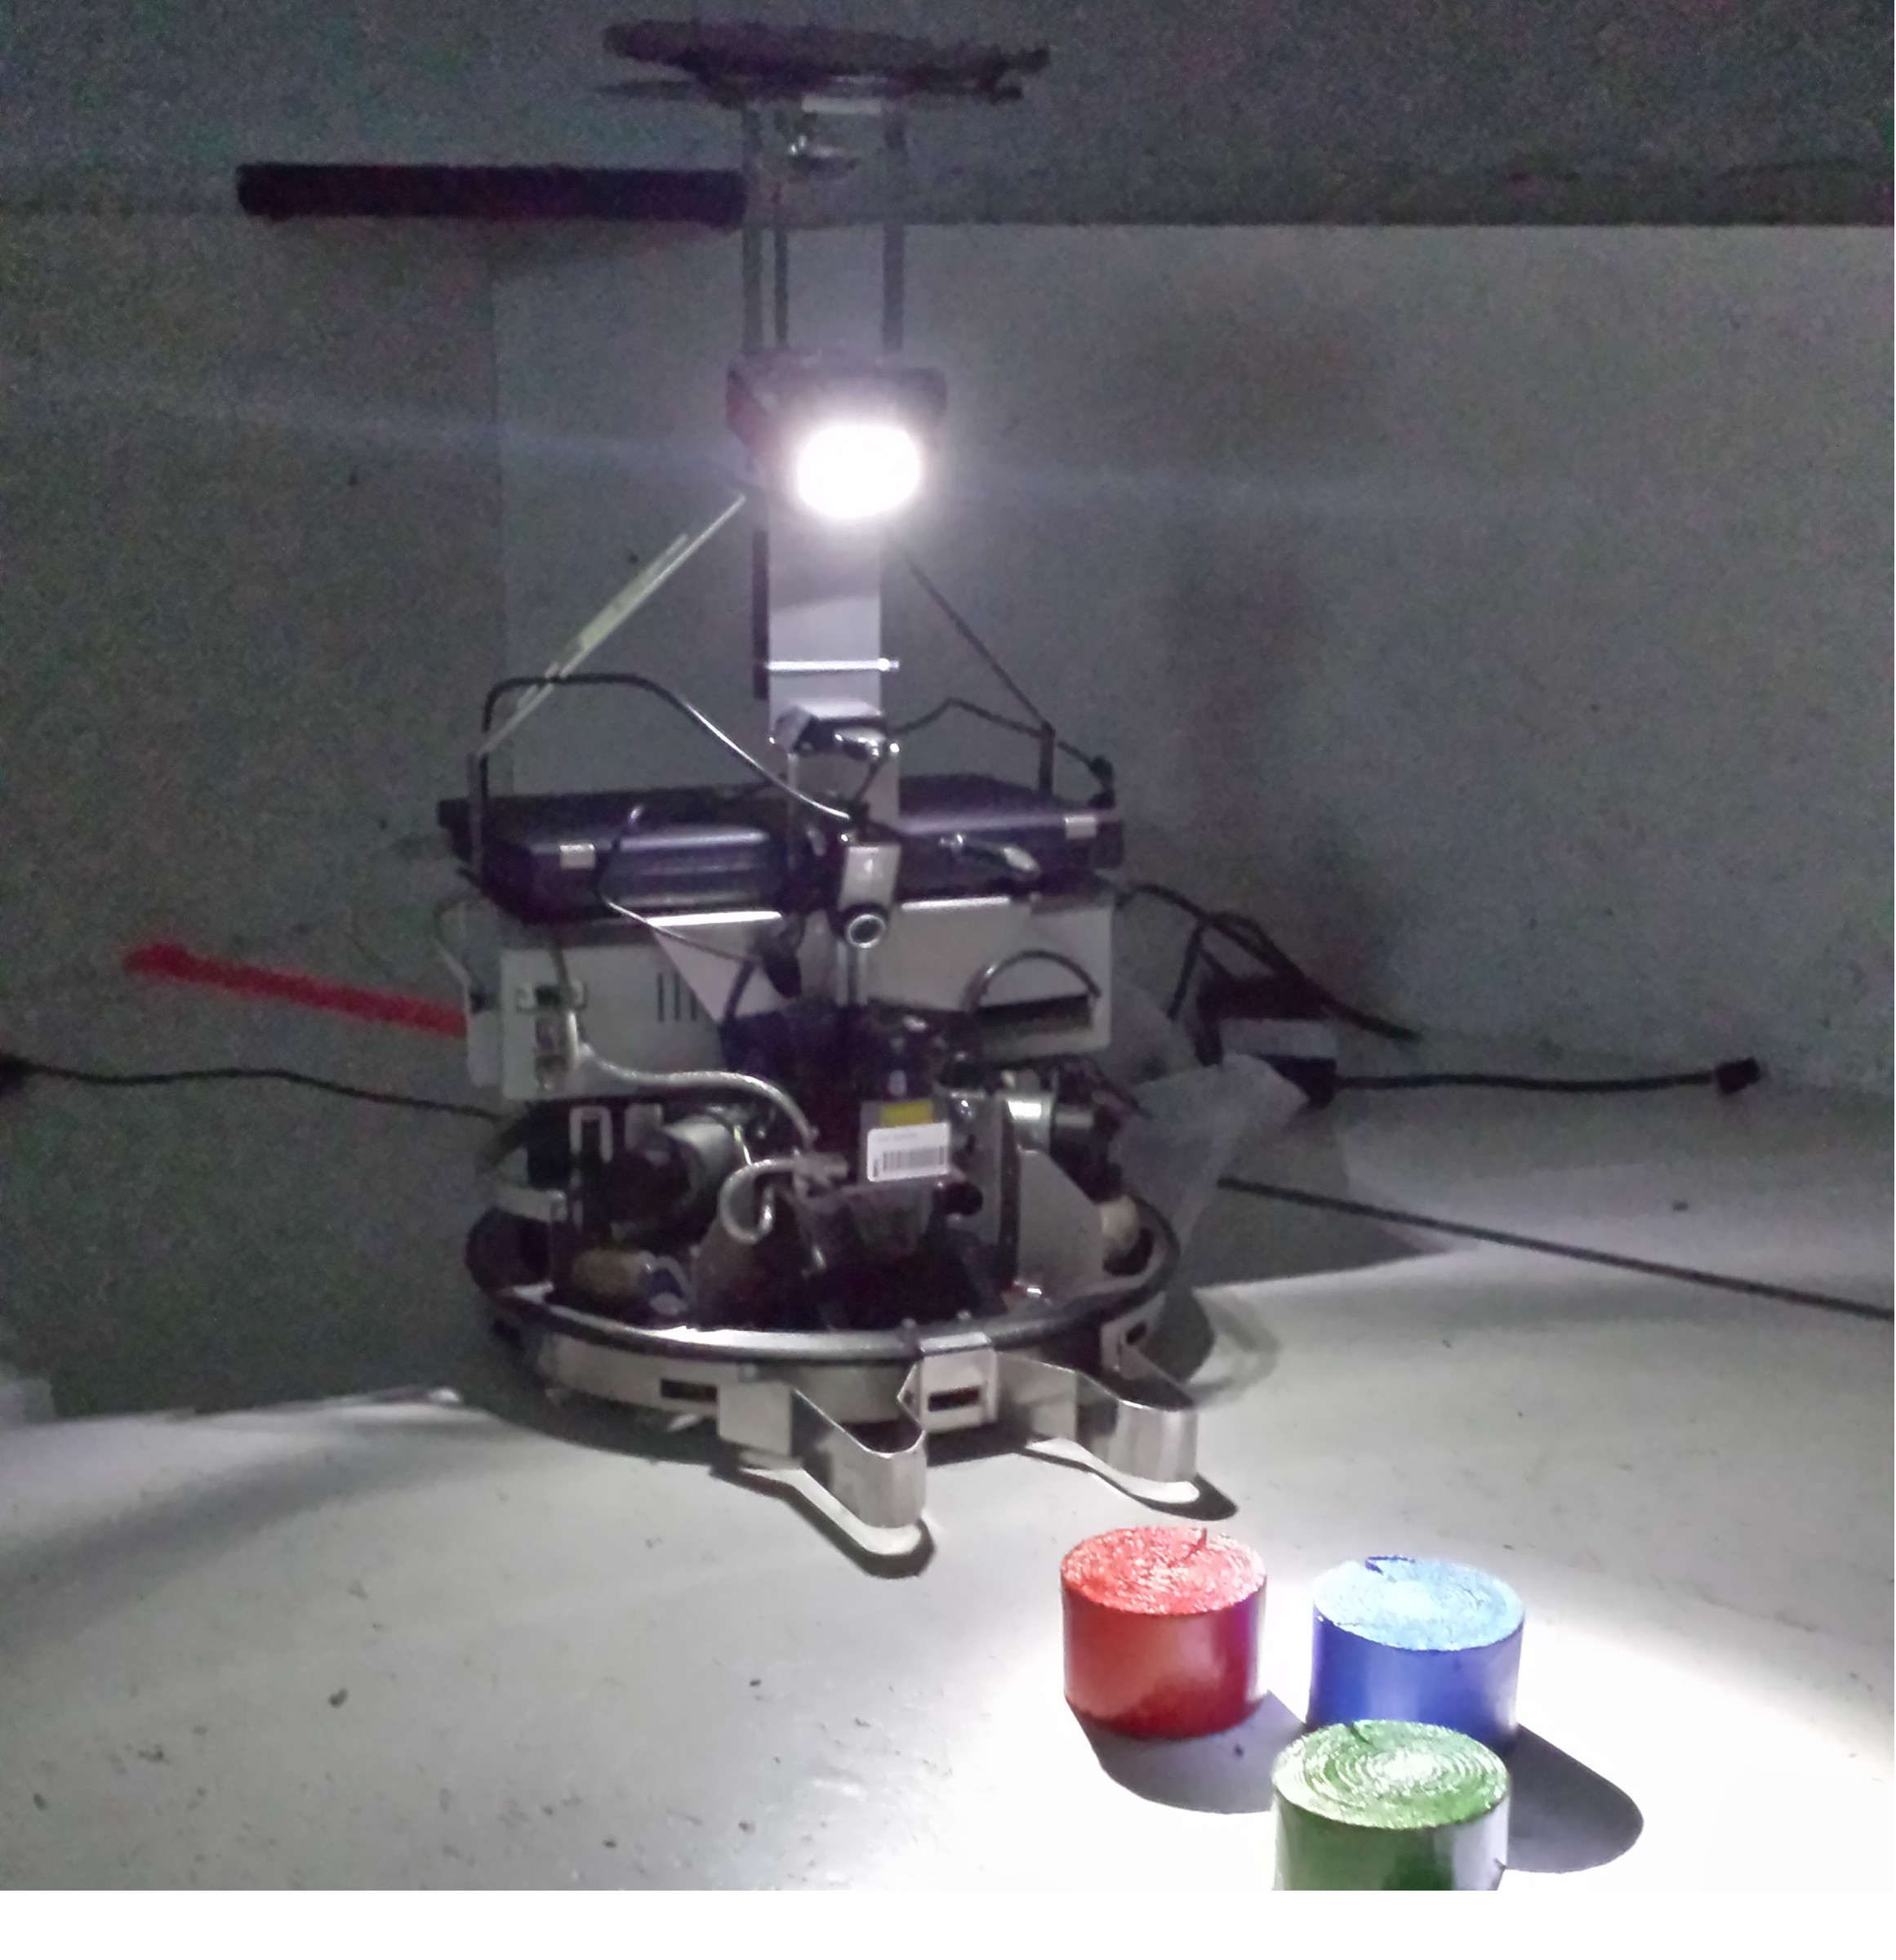
\includegraphics[width=\textwidth]{pics/hackathon_real_de}
    \caption{The Robotino has to find pucks with a webcam and bring them in a safe area.}
    \label{fig:hackathon_real}
  \end{subfigure}
  \begin{subfigure}[b]{0.48\textwidth}
    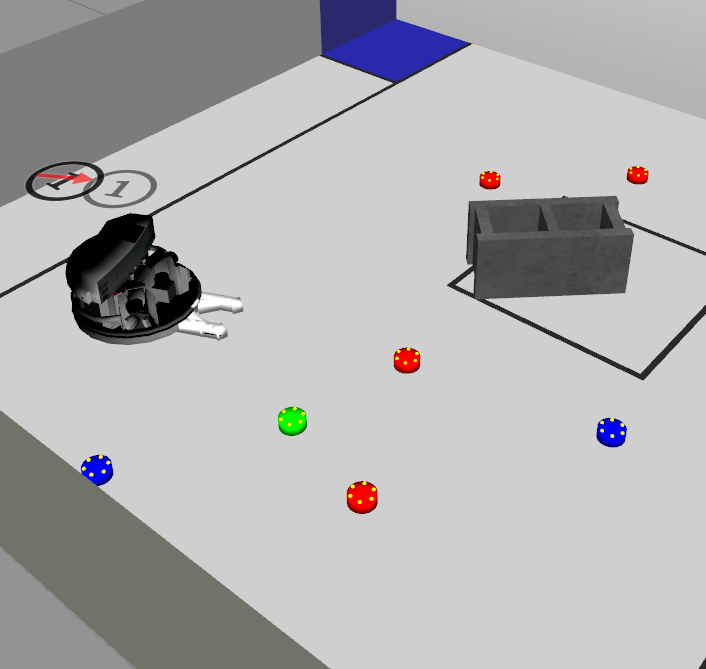
\includegraphics[width=\textwidth]{pics/hackathon_sim}
    \caption{Same scene in the simulation\\}
    \label{fig:hackathon_sim}
  \end{subfigure}
  \caption{Bonding Hackathon 2013}
  \label{fig:hackathon}
\end{figure}
We also used our simulation in the Hackathon in November 2013. The Hackathon was an event organized by Bonding\footnote{Boning is a student association which organizes events to provide insights into the working life and contacts to companies looking for employees (\url{http://www.bonding.de}).} and Carologistics. In one night, the participants got an insight into developing skills \textcolor{red}{(behavior engine in background)} with Fawkes and LUA in a search and rescue scenario. The task was to find colored pucks with the Robotino at night and bring the pucks to a safe area. Figure~\ref{fig:hackathon_real} shows a Robotino doing this task. In addition to the equipment in LLSF, the Robotino holds a flashlight and a webcam looking downwards to detect pucks. The simulation was an essential part of the Hackathon for multiple reasons. There were about 40 participants, which worked in teams of two or three people, and only 4 available Robotinos and fields. Therefore, the simulation was necessary to provide the possibility of frequently testing and testing was important because the participants had no experience with LUA, the Robotino and our behavior engine. The scripts allowed easy and fast starting of the simulation and all needed components to operate the simulated Robotino. So, the participants did not need to know how to start Gazebo, ROS and Fawkes with additional plugins. Furthermore, the simulation provided a safe environment where no hardware can be damaged. The successful use of the simulation at the Hackathon also shows the capabilities of the simulation. Many teams primarily tested their code in the simulation and added only slight changes after testing on the real robot. This shows that the simulation is very similar to the real application. Feedback from some participants showed that the simulator is easy to use and runs with a high simulation speed close to real time even on a slow notebook. We were able to increase the simulation speed because the Hackathon task did not require so much physical accuracy as the LLSF task. However, the GUI of the simulator reacted more slowly than on faster computers. We think this was due to missing graphic drivers.\\
The use of the simulation at the Hackathon also showed that the simulation is extendable and easy to modify. The new approach to detect pucks with different colors works well with the webcam module developed for machine light detection and modifying the scripts and  models for the Robotino and the LLSF field with colored pucks and obstacles was easy and fast. We also deactivated the modules and plugins we did not need in the Hackathon to save performance.\\
The Hackathon was successful, most teams were able to develop a working skill which saved multiple pucks in the final competition on the real robot although they worked the first time with LUA, the Robotino and the behavior engine. Some teams performed very well and saved nearly all pucks.

\subsection{Limitations}
In this subsection, we describe the limitations of the simulation. First of all, a simulation can not substitute testing with a real robot completely because the reality is too complex to simulate it exactly. It is especially difficult to simulate realistic physics and graphics. Because of that, we were not able to appropriately simulate omni-directional wheels with realistic odometry errors and reflections on machine lamps which cause problems for machine light recognition. Furthermore, the available performance on current computers limits the number of simulated robots and sensor update rate and precision at a reasonable simulation speed and physical accuracy. Unfortunately, some limitations of the simulation of low level sensors and actuators also restrict the possibility to test components on a higher level with dependencies on these low level components. For example we can not the reaction of the navigation on a realistic odometry error. We only can introduce an artificial odometry error. A limitation of our automated simulation run is the human interaction in the multi-robot system. In LLSF, teams can remove misbehaving robots from the game and restart a robot a single time. This can only be done in the automated tests if a human is present all the time. As we show in this thesis, we were able to develop a useful and sufficiently realistic simulation inside all these limits.\\

\section{Multi-Robot Strategies}
\label{sec:multi_robot_strategies}
In this section, we evaluate our multi-robot system and the improvements we made with the simulation. This shows what the simulation can evaluate and where we have to improve our system in the future. We compare the improved system to the version at the RoboCup 2013 in Eindhoven. As mentioned in section~\ref{sec:multi_agent_strategies}, we used two Robotinos, one with the P3-role and one with the P1P2-role. Unfortunately, the real performance in Eindhoven is not suitable for comparison with simulation runs because of the human interaction with misbehaving robots in the real game and less wrong perception results in the simulation. Furthermore, we also applied small improvements to the system that cause the system to perform better than in Eindhoven. Therefore, we rather use simulation runs with the same configuration as in Eindhoven as a basis for comparison.
\begin{figure}
  \centering
  \begin{tikzpicture}
    \begin{axis} [[
          enlarge x limits=0.5,
          xtick=data,
          height=0.7\textwidth,
          width=\textwidth,
          symbolic x coords={Eindhoven,P1P2-P3,P3-P3,P1P2-P3-R,P1P2-P3-D,P1-P2-RD},
          table/header=false,
          ylabel=Points
        ]
        \addplot [box plot median] table {evaluation.dat};
        \addplot [box plot box] table {evaluation.dat};
        \addplot [box plot top whisker] table {evaluation.dat};
        \addplot [box plot bottom whisker] table {evaluation.dat};
    \end{axis}
  \end{tikzpicture}
  \caption{The box-plots show the amount of points reached in multiple LLSF simulation runs with two robots. \textit{Eindhoven} shows the real performance at the RoboCup 2013, all other results were simulated. The labeling marks used roles and improvements (R: recycling, D: dynamic role change). Each configuration was tested ten times.}
  \label{fig:eval_two}
\end{figure}
Figure~\ref{fig:eval_two} shows the performances with two robots. We simulated 10 to 15 runs for each configuration. All experiments in the simulation have in common that there are more outliers with poor performance because we can not restart misbehaving robots in the simulation. This also scatters the performance of single simulation runs because the amount of lost points caused by a misbehaving robot depends on the time when the misbehaving starts. Some of the most common causes for bad performances are shown in Figure~\ref{fig:fails}.
\begin{figure}
  \centering
  \begin{subfigure}[b]{0.40\textwidth}
    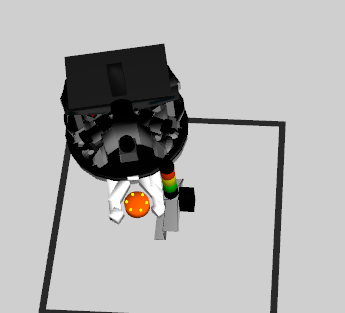
\includegraphics[width=\textwidth]{pics/bad_performance_eindhoven_no_reset}
    \caption{The Robotino wants to turn left, but can not reach the target position because of the machine.}
    \label{fig:fails_stuck}
  \end{subfigure}
  \begin{subfigure}[b]{0.40\textwidth}
    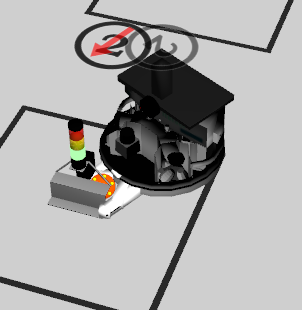
\includegraphics[width=\textwidth]{pics/wrong_local_bad_angle}
    \caption{Stuck Robotino after approaching the machine from an inappropriate angle}
    \label{fig:fails_angle}
  \end{subfigure}
  \begin{subfigure}[b]{0.40\textwidth}
    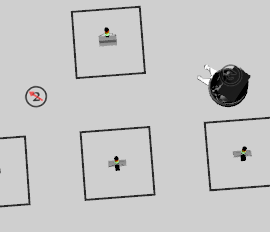
\includegraphics[width=\textwidth]{pics/p1_p2_wrong_localization_block_ins}
    \caption{The Robotino is wrongly localized and can not reach the destination.}
    \label{fig:fails_localization}
  \end{subfigure}
  \begin{subfigure}[b]{0.40\textwidth}
    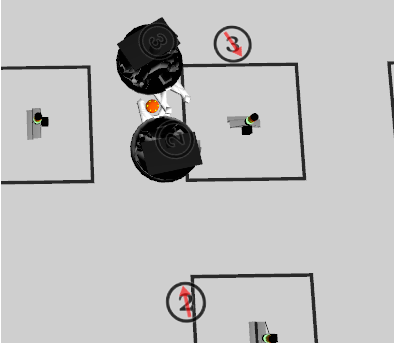
\includegraphics[width=\textwidth]{pics/crash_p3_p3_wrong_localization}
    \caption{Robotinos having troubles passing each other.}
    \label{fig:fails_passing}
  \end{subfigure}
  %% \begin{subfigure}[b]{0.48\textwidth}
  %%   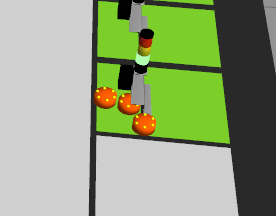
\includegraphics[width=\textwidth]{pics/p1p2_p3_d_delivery_messed}
  %%   \caption{Same scene in the simulation}
  %%   \label{fig:hackathon_sim}
  %% \end{subfigure}
  \caption{Failures and problems causing bad performance}
  \label{fig:fails}
\end{figure}
Figures~\ref{fig:fails_stuck} and~\ref{fig:fails_angle} show situations in which the Robotino gets stuck during low level movement. Often these situations block the robots the rest of the game because there is no timeout to detect that the robot is stuck or the recovery method is not able to solve the situation. These situations have a large impact on the performance of the system. The situations shown in Figure~\ref{fig:fails_localization} and~\ref{fig:fails_passing} happen during navigation. Often, such situations get solved, but it can take much time. These situations also can block the whole multi-robot system if one of the involved robots locks a position other robots need too.\\
Because these problems limit the possibilities of the system and therefore the impact of agent improvements, good runs of different configurations are more meaningful when comparing different agents.\\
As we can see in Figure\ref{fig:eval_two}, two P3 agents perform better than one P1P2 and one P3 agent. This is due to the fact that P3 provides more points per production step and is less likely to fail because of the lower amount of steps needed to finish a P3 puck. We did not use two P3 agents at the RoboCup in Eindhoven although this was already possible. We simply were not able to test it because all testing time was needed for components on a lower level. This again shows how useful the simulation is for evaluation.

\subsection{Dynamic Role Change}
We expected that the \textit{P1P2-P3-D} configuration performs 10 to 20 points better per run than the \textic{P1P2-P3} configuration because after finishing the first complex product the P1P2 agent becomes a second P3 agent. Surprisingly, the performance of P1P2-P3-D is not better than the performance of P1P2-P3. The reconstructions of the simulated P1P2-P3-D runs show that a role change happens late and only rarely because it takes a large part of the game-time to finish the complex product and when the P1P2 agents gets stuck, it happens often in a way shown above and therefore the role change does not happen. The effects of the dynamic role change on the \textit{P1-P2-RD} configuration is similar. The statistics about the produced and delivered pucks show that the change worked in $30\%$ of the games and provided 10 to 30 additional points.\\
Overall the dynamic role change has potential that is limited by the slow production speed and situations in which the robot gets completely stuck.

\subsection{Recycling}
The \textit{P1P2-P3-R} configuration mostly performs better than the P1P2-P3 configuration. The statistics show that the P1P2 agent scores 5 to 10 additional points via recycling. The first 5 recycling points are scored early in the game after the S2 production and further recycling points depend on the finished production of a complex product. The reconstructions of some simulation runs, especially with three robots, show that the recycling helps to avoid the bottleneck at the insertion area where robot get new S0 pucks. However, Figure~\ref{fig:eval_two} shows that there also are a couple of games with a worse performance than P1P2-P3. The reason is that the recycling step is more likely to fail than just getting a new S0 puck. There are cases in which the Robotino gets stuck at a machine when trying to grep a consumed puck and in which the Robotino has problems with leaving the recycle machine. In no simulated game the recycling was necessary because of S0 pucks running out of stock. This might change in the future if we can produce more and faster.

\subsection{Role Configurations for Three Agents}
To find a good role assignment for three robots and figure out the problems we need to tackle in the future, we compare several configurations here. Figure~\ref{fig:eval_three} shows the evaluation results with the configurations \textit{P1P2-P3-P3-RD}, \textit{P1-P2-P3-RD} and \textit{P3-P3-P3}.
\begin{figure}
  \centering
  \begin{tikzpicture}
    \begin{axis} [[
          enlarge x limits=0.5,
          xtick=data,
          height=0.7\textwidth,
          width=\textwidth,
          symbolic x coords={P1P2-P3-P3-RD,P1-P2-P3-RD,P3-P3-P3},
          table/header=false,
          ylabel=Points
        ]
        \addplot [box plot median] table {evaluation_3.dat};
        \addplot [box plot box] table {evaluation_3.dat};
        \addplot [box plot top whisker] table {evaluation_3.dat};
        \addplot [box plot bottom whisker] table {evaluation_3.dat};
    \end{axis}
  \end{tikzpicture}
  \caption{The box-plots show the amount of points reached in multiple LLSF simulation runs with three robots. The labeling and test population is equivalent to Figure~\ref{fig_eval_two}.}
  \label{fig:eval_three}
\end{figure}
Surprisingly, no configurations with three robots performs better than a similar configuration with two robots. The reasons can easily be seen in some reconstructions. First, using three robots lead to significantly more navigation conflicts, such as in Figure~\ref{fig:fails_passing}, than using two robots. This often also effects the third robot when it has to pass the other two robots or it needs a resources that is locked by another robot. Second, the bottleneck of the current approach, which is the single point for getting new pucks, affects three robots more than two. Therefore, robots often have to wait until for other robots. Third, the failure of single robots remains a big problem. On the one hand, there are two robots left if one fails, but on the other hand a failing robot that locked an important resource still blocks the whole system.

\subsection{Different Abstraction Levels}
\textcolor{red}{bad network influence eval}



